\documentclass[../../main.tex]{subfiles}

\graphicspath{{../../image/}{../../figure/}}

\begin{document}

\section{习题}\label{section:ch18-习题}

\begin{exercise}\label{exercise:ch18-01}
（$\star\star$）考虑变换 $\bm{x}=\bm{f}(\bm{z})$ 及其逆变换 $\bm{z}=\bm{g}(\bm{x})$。通过对 $\bm{x}=\bm{f}(\bm{g}(\bm{x}))$ 进行求导，证明
\begin{align}
  \bm{J}\bm{K}=\bm{I},\label{align:ch18-习题01-JK}
\end{align}
其中 $\bm{I}$ 是单位矩阵，$\bm{J}$ 和 $\bm{K}$ 则是元素分别为如下矩阵
\begin{align}
  J_{ij}=\frac{\partial g_i}{\partial x_j}\quad\text{和}\quad K_{ij}=\frac{\partial f_i}{\partial z_j}\label{align:ch18-习题01-JK定义}
\end{align}
的矩阵。利用矩阵乘积的行列式是矩阵各自行列式的乘积这一结论，证明
\begin{align}
  \det(\bm{J})=\frac{1}{\det(\bm{K})}.\label{align:ch18-习题01-行列式}
\end{align}
然后证明密度在变量变换下的转换公式［\eqref{align:ch18-change-var}］可以重写为
\begin{align}
  p_x(\bm{x})=p_z\big(\bm{g}(\bm{x})\big)\left|\det\bm{K}\right|^{-1},\label{align:ch18-习题01-密度}
\end{align}
其中 $\bm{K}$ 是在 $\bm{z}=\bm{g}(\bm{x})$ 处进行计算的。
\end{exercise}

\begin{exercise}\label{exercise:ch18-02}
（$\star$）考虑一个由形式如下的可逆变换序列构成的变换：
\begin{align}
  \bm{x}=\bm{f}_1\big(\bm{f}_2(\cdots\bm{f}_{M-1}(\bm{f}_M(\bm{z}))\cdots)\big).\label{align:ch18-习题02-复合}
\end{align}
证明其逆函数由下式给出：
\begin{align}
  \bm{z}=\bm{f}_M^{-1}\big(\bm{f}_{M-1}^{-1}(\cdots\bm{f}_2^{-1}(\bm{f}_1^{-1}(\bm{x}))\cdots)\big).\label{align:ch18-习题02-逆}
\end{align}
\end{exercise}

\begin{exercise}\label{exercise:ch18-03}
（$\star$）考虑形式如下的线性变量变换：
\begin{align}
  \bm{x}=\bm{z}+\bm{b}.\label{align:ch18-习题03-平移}
\end{align}
证明此变换的 Jacobian 矩阵是单位矩阵。通过对 $\bm{z}$ 空间中一个小区域的体积与 $\bm{x}$ 空间中对应区域的体积进行比较，解释这一结果。
\end{exercise}

\begin{exercise}\label{exercise:ch18-04}
（$\star\star$）证明\eqref{align:ch18-maf逆}给出的自回归标准化流变换的 Jacobian 矩阵是一个下三角矩阵。矩阵的行列式由主对角线上项的乘积给出，因此容易计算。
\end{exercise}

\begin{exercise}\label{exercise:ch18-05}
（$\star$）考虑残差网络的前向传播方程［\eqref{align:ch18-残差}］，并考虑时间变量 $t$ 的一个小的增量：
\begin{align}
  \bm{z}^{(t+\varepsilon)}=\bm{z}^{(t)}+\varepsilon\bm{f}\big(\bm{z}^{(t)},\bm{w}\big),\label{align:ch18-习题05-增量}
\end{align}
来自神经网络的加性贡献被 $\varepsilon$ 缩放。注意\eqref{align:ch18-残差}对应于 $\varepsilon=1$ 的情况。通过取极限 $\varepsilon\to0$，推导出\eqref{align:ch18-神经ode}所示的前向传播微分方程。
\end{exercise}

\begin{exercise}\label{exercise:ch18-06}
（$\star\star$）在这个习题和下一个习题中，我们将为神经 ODE 的反向传播方程和梯度计算方程提供非正式的推导。对于这些结果更正式的推导可以在 Chen et al. (2018) 中找到。写出与前向传播方程［\eqref{align:ch18-习题05-增量}］相对应的反向传播方程。通过取极限 $\varepsilon\to0$，推导出反向传播方程［\eqref{align:ch18-伴随方程}］，其中 $\bm{a}(t)$ 由\eqref{align:ch18-伴随}定义。
\end{exercise}

\begin{exercise}\label{exercise:ch18-07}
（$\star\star$）利用\eqref{align:ch08-权重梯度}，写出损失函数 $L(\bm{z}(T))$ 的梯度表达式，该损失函数针对的是\eqref{align:ch18-习题05-增量}定义的多层残差网络，其中所有层共享相同的参数向量 $\bm{w}$。通过取极限 $\varepsilon\to0$，推导出计算损失函数导数的方程［\eqref{align:ch18-参数梯度}］。
\end{exercise}

\begin{exercise}\label{exercise:ch18-08}
（$\star\star$）在这个习题中，我们将为\eqref{align:ch18-瞬时变量替换}的一维版本提供非正式的推导。考虑时间 $t$ 的分布 $q(z)$，从 $z$ 到 $x$ 的变换在时间 $t+\delta t$ 变成了新的分布 $p(x)$。同时考虑附近值 $z$ 和 $z+\Delta z$ 以及相应的值 $x$ 和 $x+\Delta x$，如\cref{figure:ch18-密度变换示意}所示。首先写出一个方程来表达区间 $\Delta z$ 中的概率质量与区间 $\Delta x$ 中的概率质量相同。然后写出一个方程来显示概率密度是如何从 $t$ 变化到 $t+\delta t$ 的，用导数 $\mathrm{d}q(t)/\mathrm{d}t$ 表示。接下来通过引入函数 $f(z)=\mathrm{d}z/\mathrm{d}t$ 写下一个关于 $\Delta z$ 的 $\Delta x$ 的方程。最后通过结合以上三个方程并取极限 $\delta t\to0$，证明
\begin{align}
  \frac{\mathrm{d}}{\mathrm{d}t}\ln q(z)=-f'(z),\label{align:ch18-习题08-一维}
\end{align}
这就是\eqref{align:ch18-瞬时变量替换}的一维版本。
\end{exercise}

\begin{figure}[htbp]
  \centering
  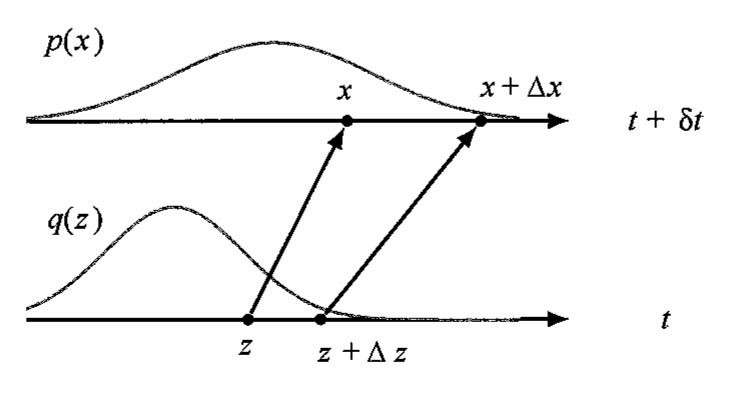
\includegraphics[width=0.62\textwidth]{ch18-fig507-density-shift.png}
  \caption{概率密度变换的示意图，用于推导一维连续标准化流的方程}
  \label{figure:ch18-密度变换示意}
\end{figure}

\begin{exercise}\label{exercise:ch18-09}
（$\star\star$）\cref{figure:ch18-连续流}中的流线是通过取一组等间距的值，并利用每个 $t$ 值处累积分布函数的逆函数，通过绘制对应的 $\bm{z}$ 空间中的点而得到的。证明这等同于使用微分方程［\eqref{align:ch18-流ode}］计算流线，其中 $\bm{f}$ 由\eqref{align:ch18-瞬时变量替换}定义。
\end{exercise}

\begin{exercise}\label{exercise:ch18-10}
（$\star\star$）使用微分方程［\eqref{align:ch18-流ode}］写下连续标准化流的基础密度表达式，该表达式以输出密度形式表示，并在 $t$ 上进行积分。利用改变定积分符号等同于交换积分限的事实，证明反转连续标准化流的计算成本与评估正向流的计算成本相同。
\end{exercise}

\begin{exercise}\label{exercise:ch18-11}
（$\star$）证明 Hutchinson 的迹估计器［\eqref{align:ch18-迹估计}］右侧的期望等于 $\operatorname{Tr}(\bm{A})$，这对任何的 $M$ 值都成立，从而证明该估计器是无偏的。
\end{exercise}

\end{document}
